\chapter{High Intensity Studies}
\label{sec:ch6}

\section{Intensity-Dependent Effects and Non-Gaussian Beam Profiles}

For this chapter, the focus goes back to the Fermilab Recycler Ring. All the experiments and measurements done in Ch. \ref{sec:ch4} were done at low intensities, i.e., less than 1e10 particles per bunch (ppb). Nevertheless, current operations and future operations under PIP-II objectives are done at higher intensities, i.e., 5e10 ppb for current operations and 8e10 ppb for PIP-II. Therefore, it is relevant to explore resonance compensation at higher intensities. 

\cite{qgaussian}

\begin{figure}[H]
    \centering
    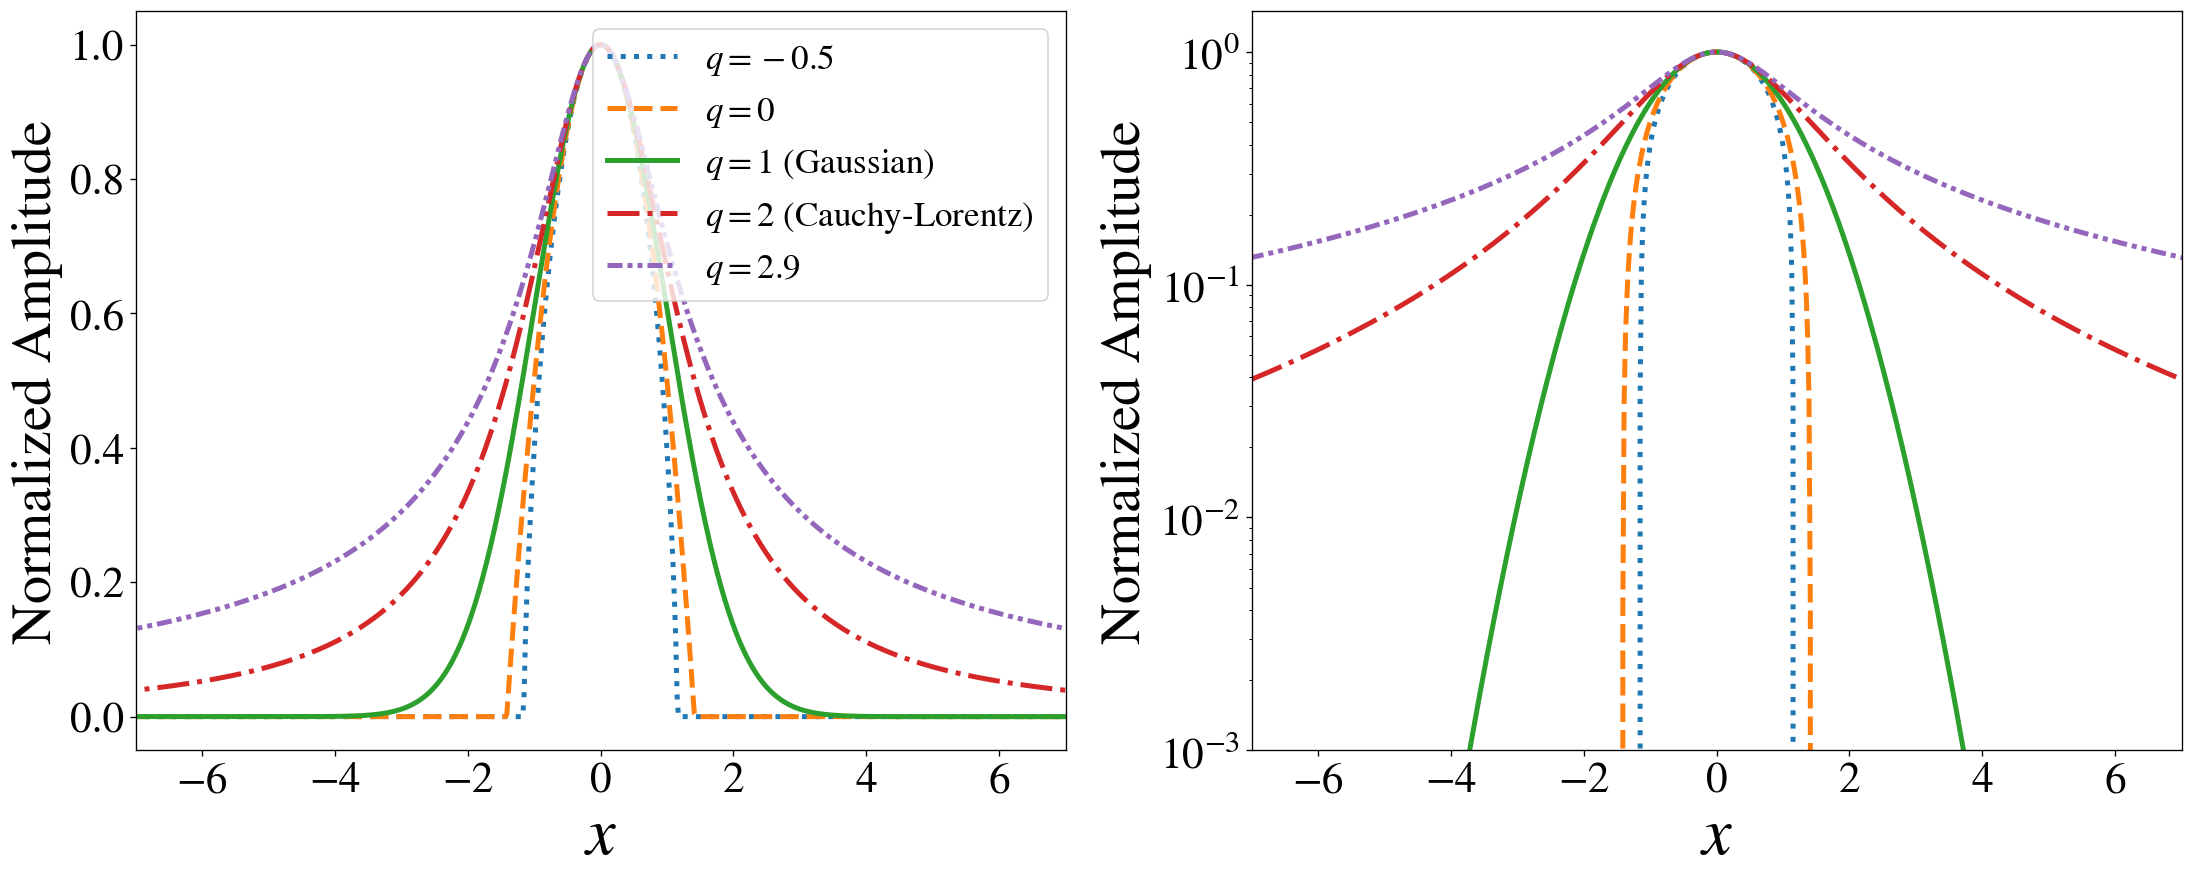
\includegraphics[width=\textwidth,keepaspectratio]{chapter6/qgaussians.png}
    \caption{Several q-Gaussian distributions for different q parameters normalized to unit amplitude and with a scale parameter of $\sigma=1$.}
    \label{fig:qgaussians}
\end{figure}

\section{Space Charge Tune Shift}

The most relevant parameter for high-intensity operation is the space charge tune shift. As mentioned in Ch. \ref{sec:ch2}, the space charge tune shift is an incoherent quantity meaning every particle will feel a different magnitude of this effect. Nevertheless, as shown in Figs. \ref{fig:rrtdmid} and \ref{fig:rrtdhigh}, this incoherent quantity will be contained within a necktie distribution. This necktie profile will define the space charge tune spread. When particles are in the beam core, they will feel the largest space charge potential, leading to the largest detuning and defining the edge of the necktie distribution.

Equation \ref{eq:scave1} showed a general way to calculate the space charge tune shift for particles at different amplitudes $J_u$. Nevertheless, this calculation is an involved process where the envelope equation has to be solved around the ring at the same time as the Poisson equation, Eq. \ref{eq:poisson1}. Different approximations can be done, in order to do rapid estimates of the space charge tune shift. Furthermore, a more important quantity is the maximum tune shift of the beam core particles. This will ultimately define the space charge tune spread. While this quantity can be calculated using PySCRDT \cite{scrdt_report}, a cruder estimate can also be calculated. This involves using a smooth-lattice approximation and circular beam pipe approximation, as used in Ref. \cite{zhang}. 

With these simplifications, the space charge tune spread can be found as:
\begin{equation}
    \label{eq:tunesc}
    \Delta Q_{u,sc}=\frac{-3 N_b r_0 R S}{4 \sigma_z \beta_L \gamma_L ^2 \varepsilon_{n,u,95\%}},    
\end{equation}
where $N_b$ is the number of protons per bunch, $r_0=1.535\times 10^{-18}$ meters is the classical radius of the proton, $\sigma_z = 0.5726$ meters is the bunch length, $R = C/(2 \pi)$ is the radius of the Recycler Ring with a circumference of $C=3319.4$ meters, $S=1.596$ is a geometrical factor of the bunch, $\varepsilon_{n,u,95\%}$ is the 95\% normalized emittance in the $u$ plane, and $(\beta_L,\gamma_L)$ are the longitudinal relativistic factors.   

\section{Measurement of Tune Spread}

Figure \ref{fig:dynamictunespread} shows slices of loss maps at different intensities. The top slice corresponds to an intensity of 2 BTs, i.e., approximately $0.6\times10^{10}$ particles per bunch. The bottom slice corresponds to an intensity of 17 BTs, approximately $6.0\times10^{10}$ ppb, which is close to the maximum intensity that can be provided by Booster in single batch. The important thing to note here is that as the intensity increases the losses happen early in the tune ramp. This can be correlated to the space charge tune spread using the location of the $3Q_x$ line, which corresponds to where all the beam is lost. For example, for the bottom slice the losses start happening at $Q_x=25.37$, while all beam is lost at $Q_x=25.345$. This means the space charge tune spread can be approximated to 0.025. Ultimately, Fig. \ref{fig:dynamictunespread} shows beams with space charge tune spreads that range from 0.005 to 0.025.

\newpage
\begin{figure}[H]
    \centering
    \includegraphics[width=\textwidth,height=0.95\textheight,keepaspectratio]{chapter6/scts_measure.png}
    \caption{Dynamic loss strips at a fixed vertical set tune of $Q_y=24.45$ and on a range from $Q_x=25.39$ to $Q_x=25.32$ for different intensities.}
    \label{fig:dynamictunespread}
\end{figure}
\newpage

Another thing to note from Fig. \ref{fig:dynamictunespread} is how the space charge tune shift tends to stabilize to a value of around 0.025 for intensities higher than 12 BTs or $4.4\times 10^{10}$. This is due to the fact that the equilibrium emittance grows exponentially at higher intensities. Specifically, Ref. \cite{betiay} shows how the beam emittance grows with intensity in the Recycler Ring. This study combined with calculations of the space charge tune shift provided in Ref. \cite{zhang}, explain this behavior. The emittance grows at the same pace as the beam intensity leading to a stable tune shift.

The maximum tune spread shown in Fig. \ref{fig:dynamictunespread} is around 0.02, which only compares to 1/5 of the PIP-II projection. It is worth pointing out, that these experiments are done for a single batch with no slip stacking. Therefore, with slip stacking and smaller beam emittance coming from Booster, space charge tune shifts in the RR of around 0.1 will be possible in the PIP-II era.  

\begin{figure}[H]
    \centering
    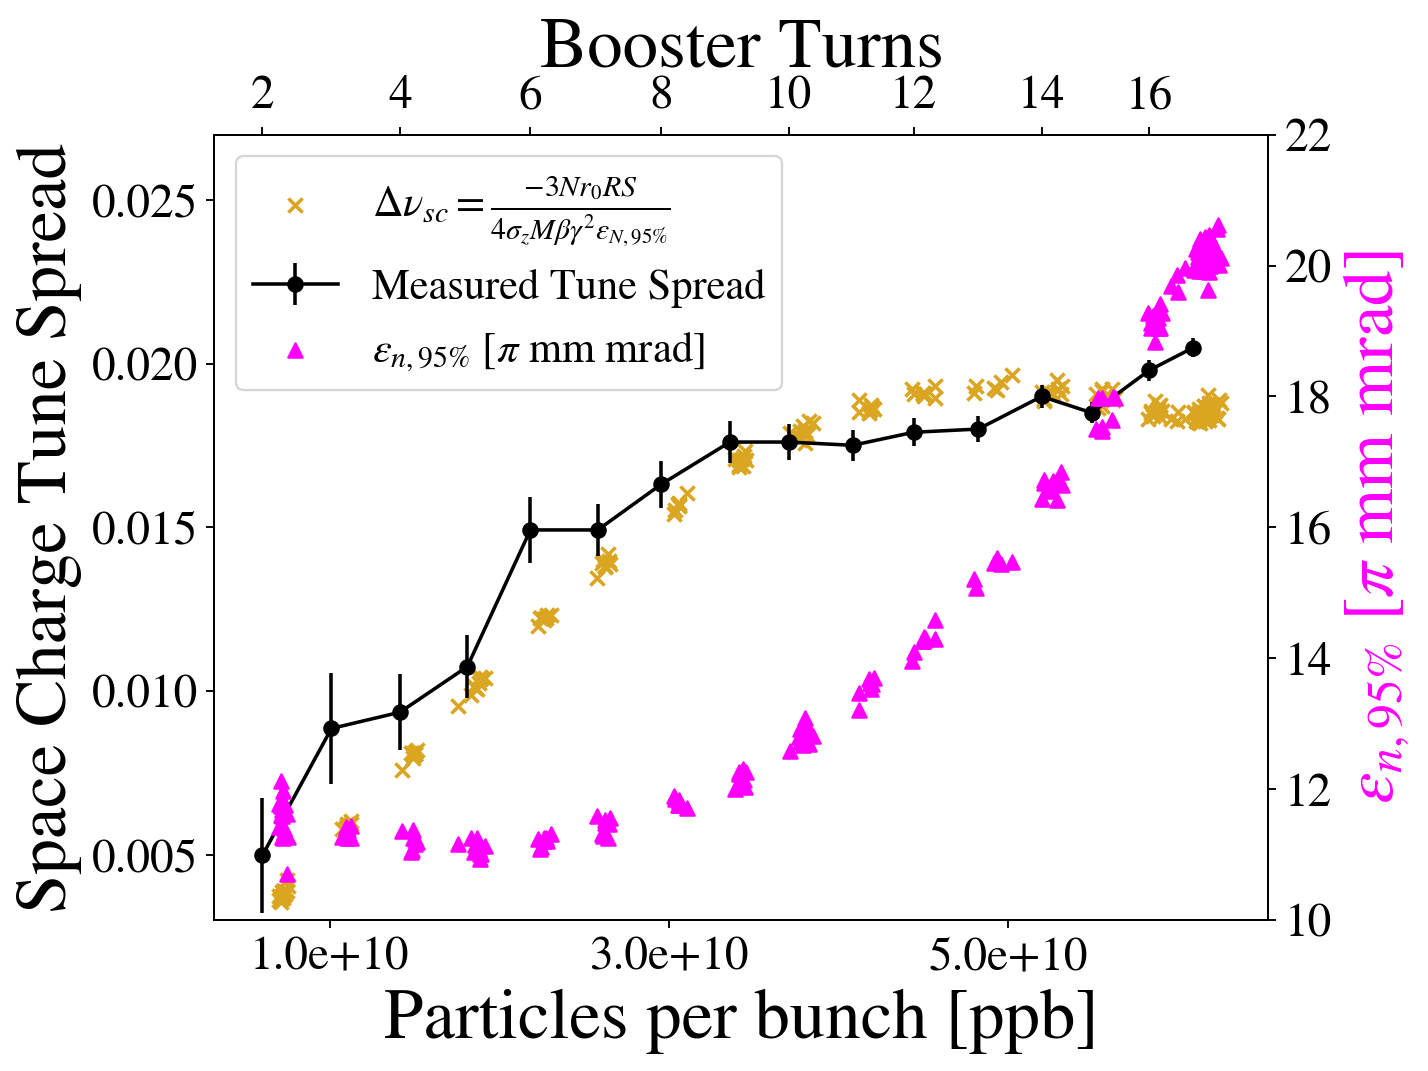
\includegraphics[width=\columnwidth]{chapter6/tune_spread.png}
    \caption{Tune spread measurements compared to tune spread calculations from horizontal emittances measured with multiwire data.}
    \label{fig:tunespread}
\end{figure}

\section{\label{sec:ch6sts}Static Tune Scans at Different Intensities}

\begin{figure}[H]
    \centering
    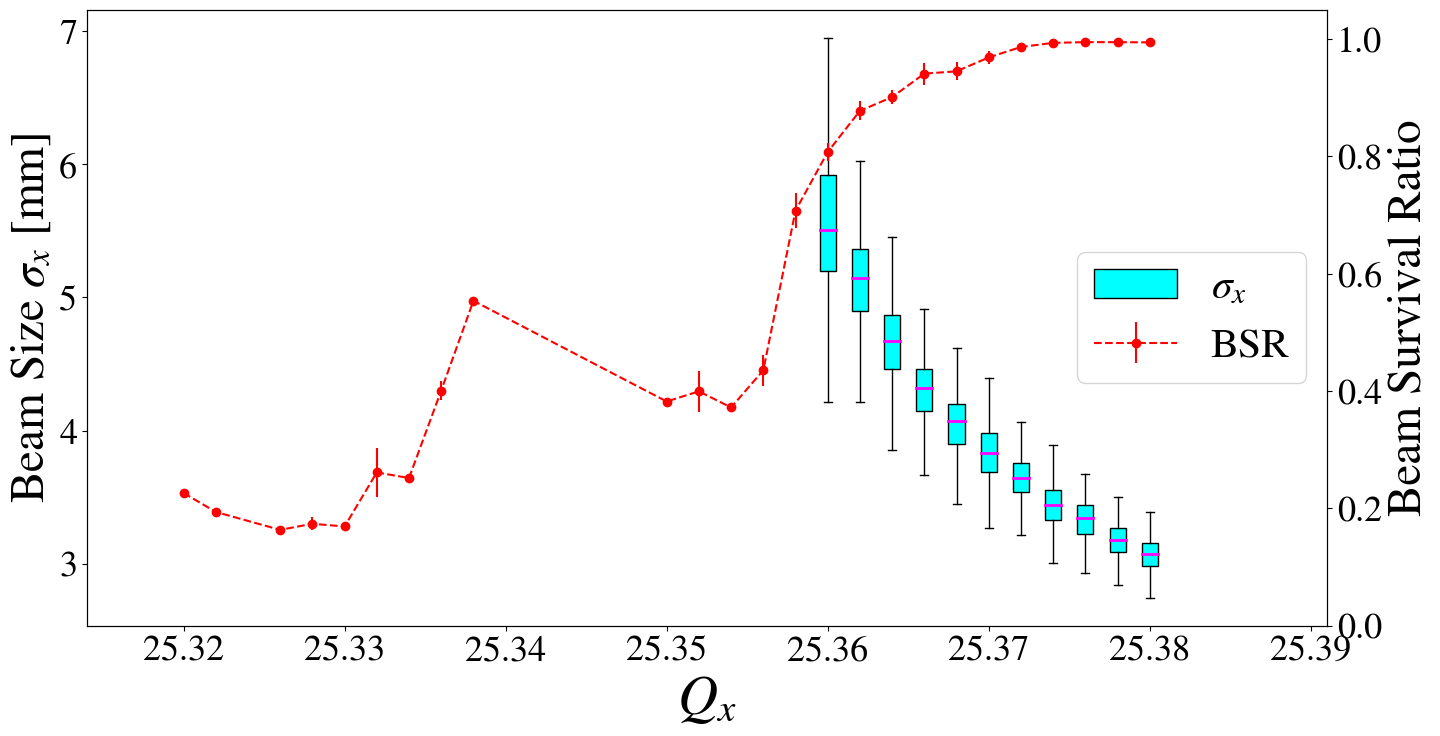
\includegraphics[width=\columnwidth]{chapter6/static14turns_BARE_dampersON.png}
    \caption{Static tune scan at an equivalent intensity of 14 Booster turns or approximately 4.5e10 ppb with no $3Q_x$ compensation and transverse dampers on.}
    \label{fig:static14_bare}
\end{figure}

\begin{figure}[H]
    \centering
    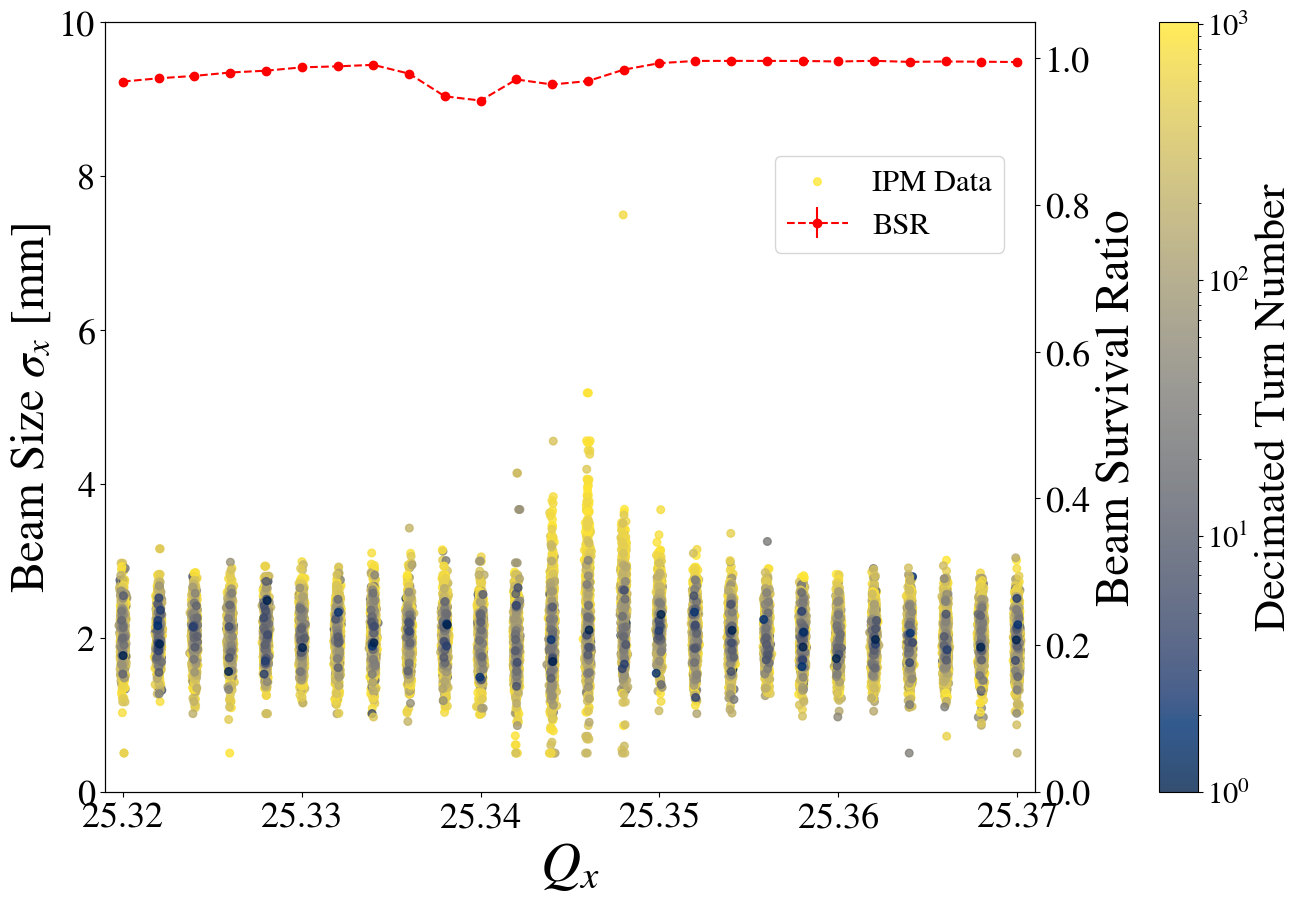
\includegraphics[width=\columnwidth]{chapter6/static2turns_dampersOFF.png}
    \caption{Static tune scan at an equivalent intensity of 2 Booster turns or approximately 0.5e10 ppb.}
    \label{fig:static2_scatter}
\end{figure}

\begin{figure}[H]
    \centering
    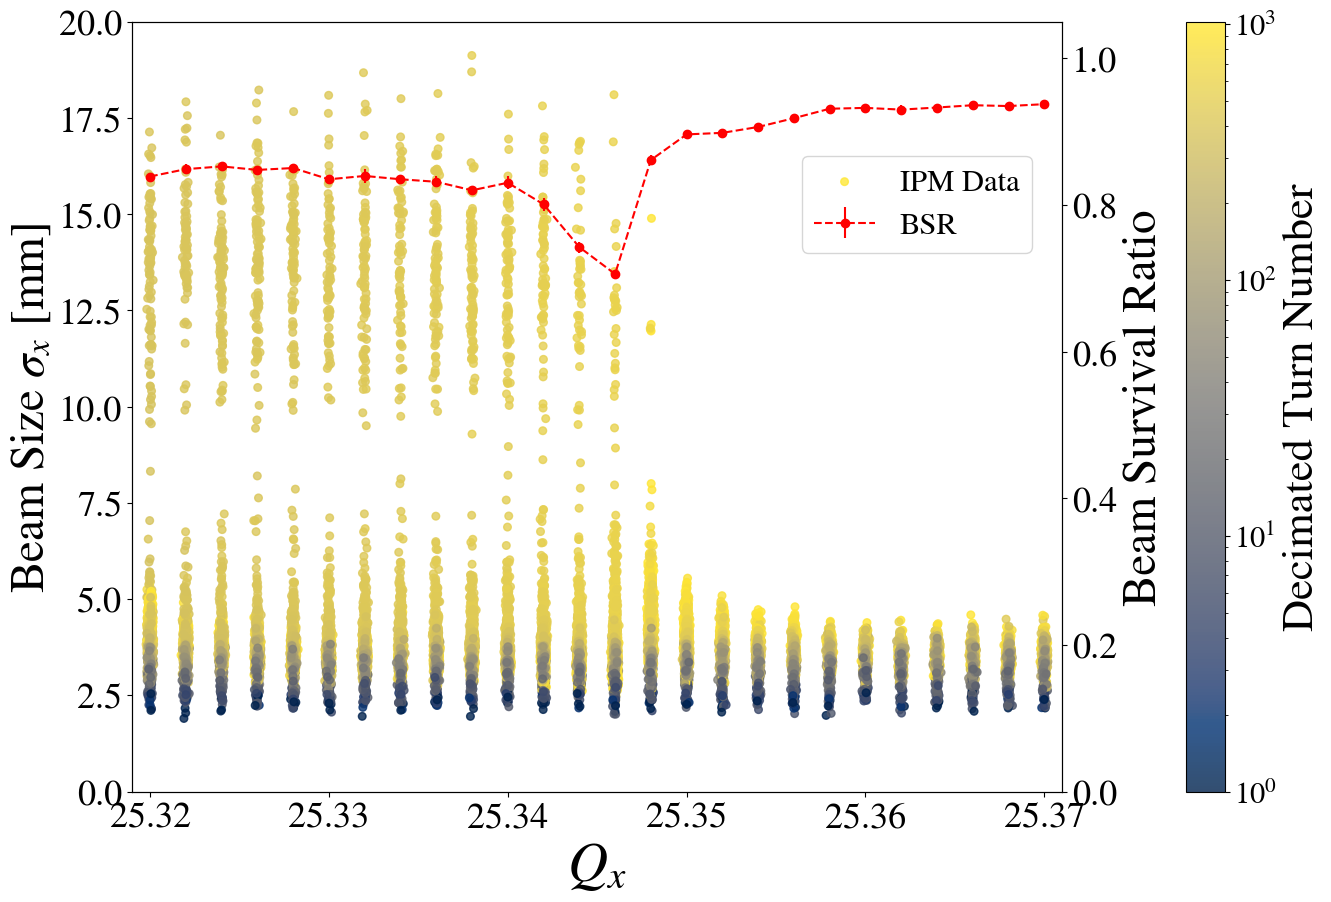
\includegraphics[width=\columnwidth]{chapter6/static8turns_dampersOFF.png}
    \caption{Static tune scan at an equivalent intensity of 8 Booster turns or approximately 3e10 ppb.}
    \label{fig:static8_scatter}
\end{figure}

\begin{figure}[H]
    \centering
    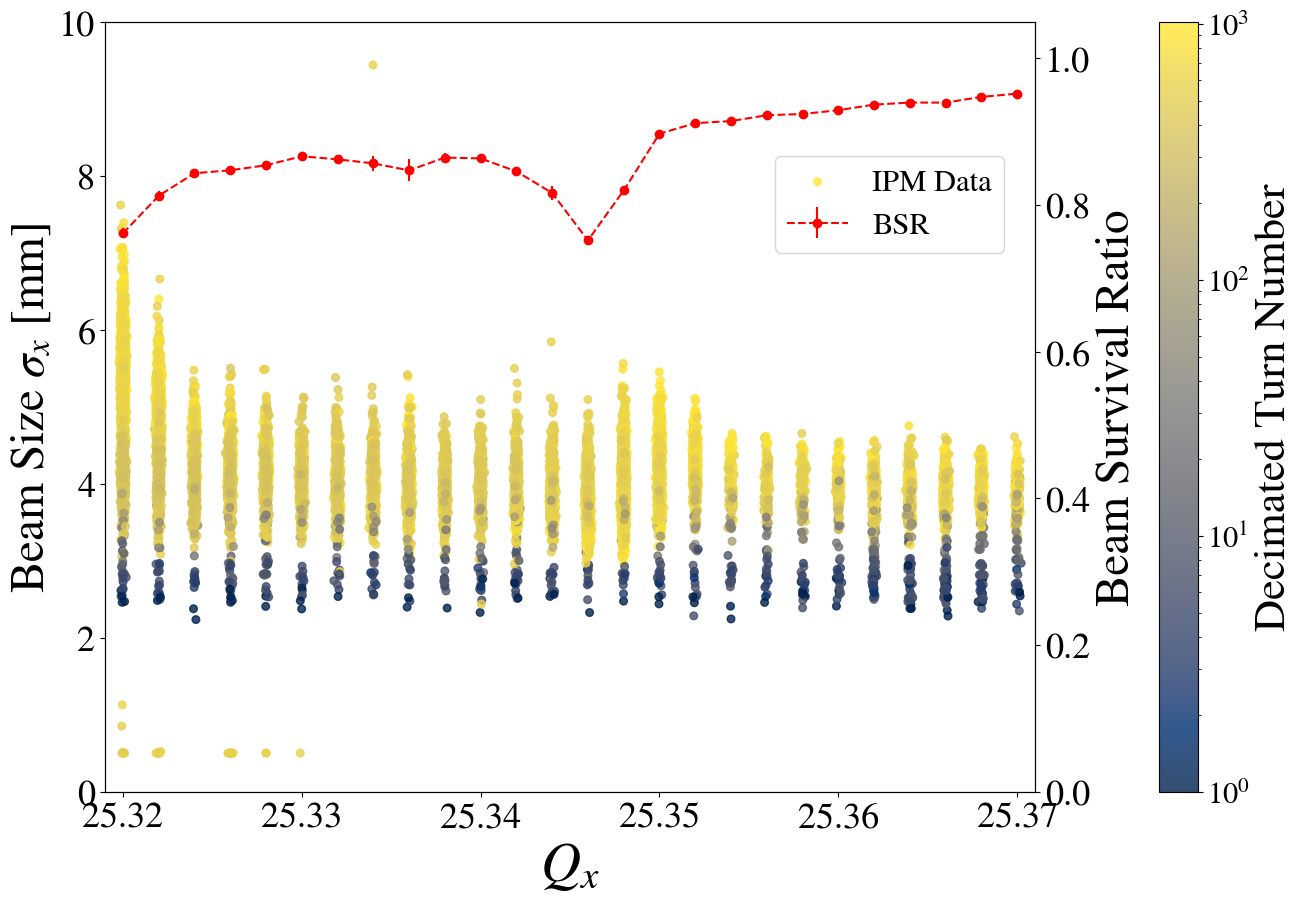
\includegraphics[width=\columnwidth]{chapter6/static14turns_dampersOFF.png}
    \caption{Static tune scan at an equivalent intensity of 14 Booster turns or approximately 4.5e10 ppb.}
    \label{fig:static14}
\end{figure}

\begin{figure}[H]
    \centering
    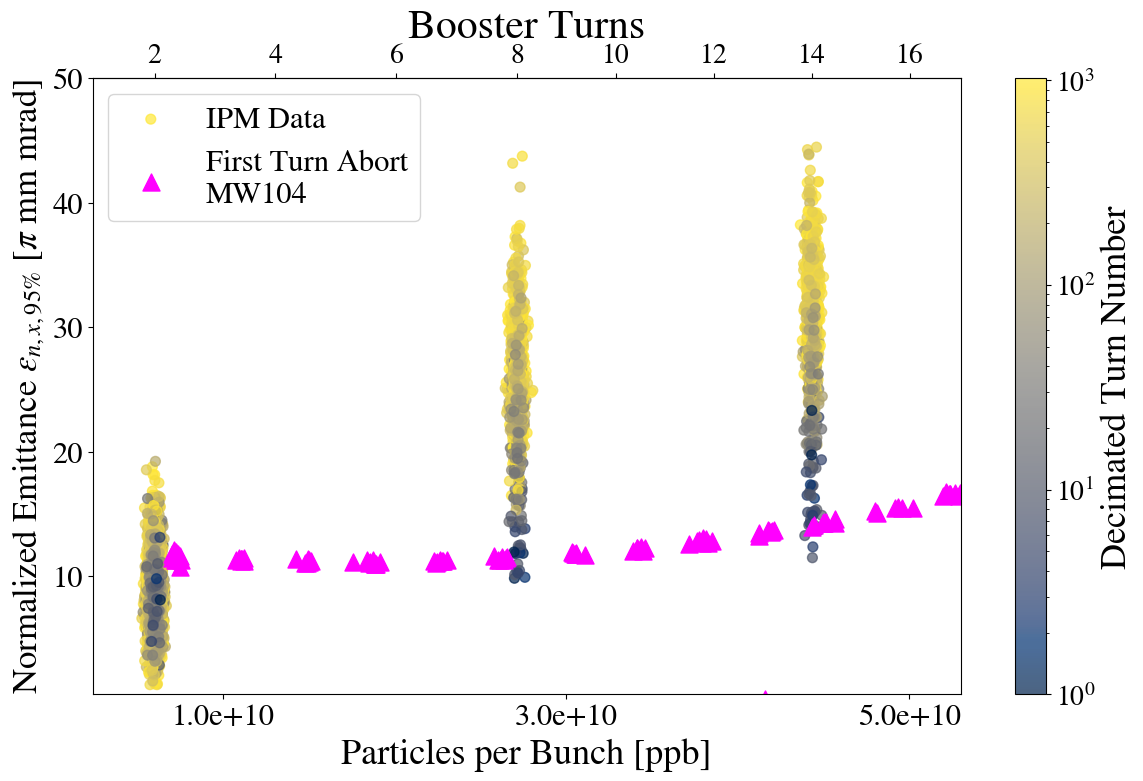
\includegraphics[width=\columnwidth]{chapter6/25370_scatter.png}
    \caption{IPM data and multi-wire first turn abort data for $Q_x=25.370$ at different intensities.}
    \label{fig:25370_scatter}
\end{figure}

\begin{figure}[H]
    \centering
    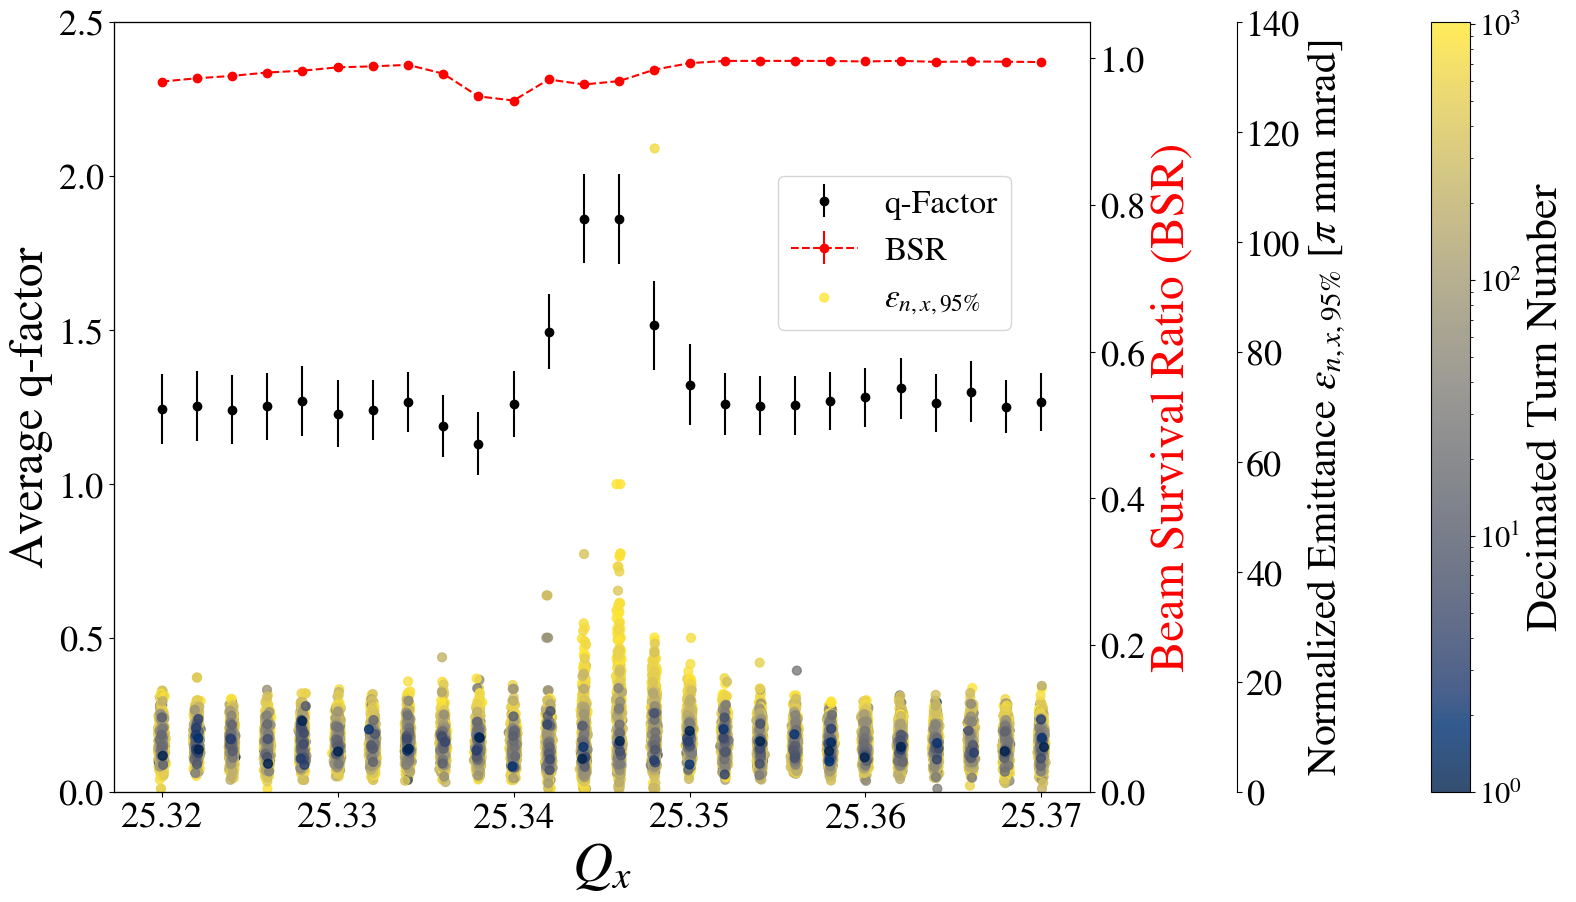
\includegraphics[width=\columnwidth]{chapter6/static2turns_emittance_dampersOFF.png}
    \caption{Static tune scan with beam survival ratio (BSR), average q-factor for the q-Gaussian fits, and beam size $\sigma_x$ at an equivalent intensity of 2 Booster turns or approximately 0.5e10 ppb.}
    \label{fig:static2_q}
\end{figure}

\begin{figure}[H]
    \centering
    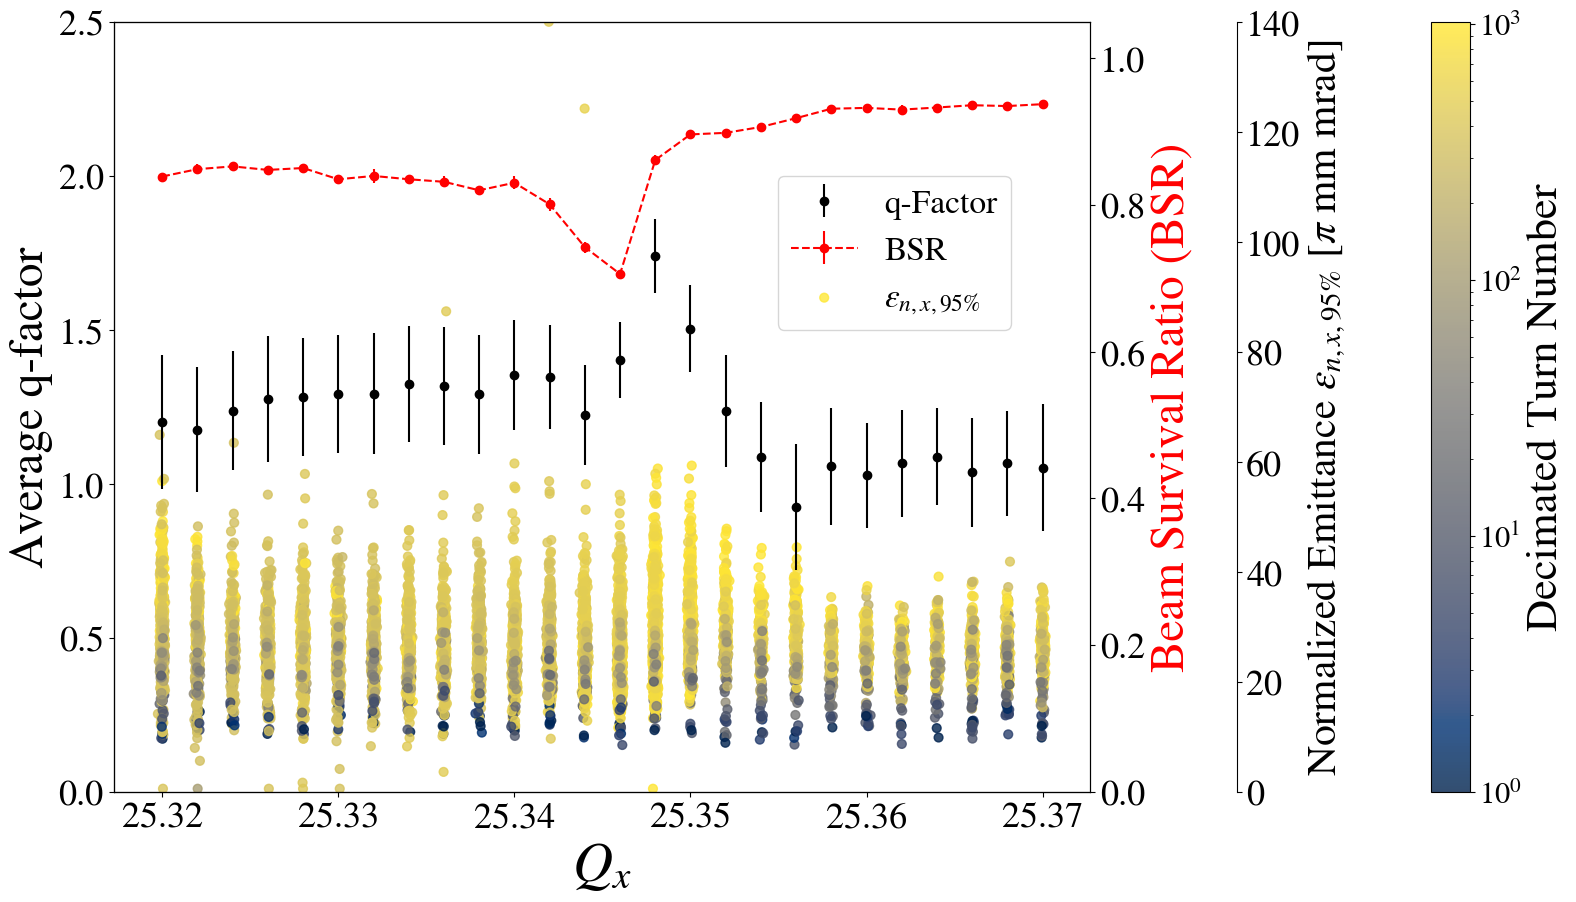
\includegraphics[width=\columnwidth]{chapter6/static8turns_emittance_dampersOFF.png}
    \caption{Static tune scan with beam survival ratio (BSR), average q-factor for the q-Gaussian fits, and beam size $\sigma_x$ at an equivalent intensity of 8 Booster turns or approximately 3e10 ppb.}
    \label{fig:static8_q}
\end{figure}

\begin{figure}[H]
    \centering
    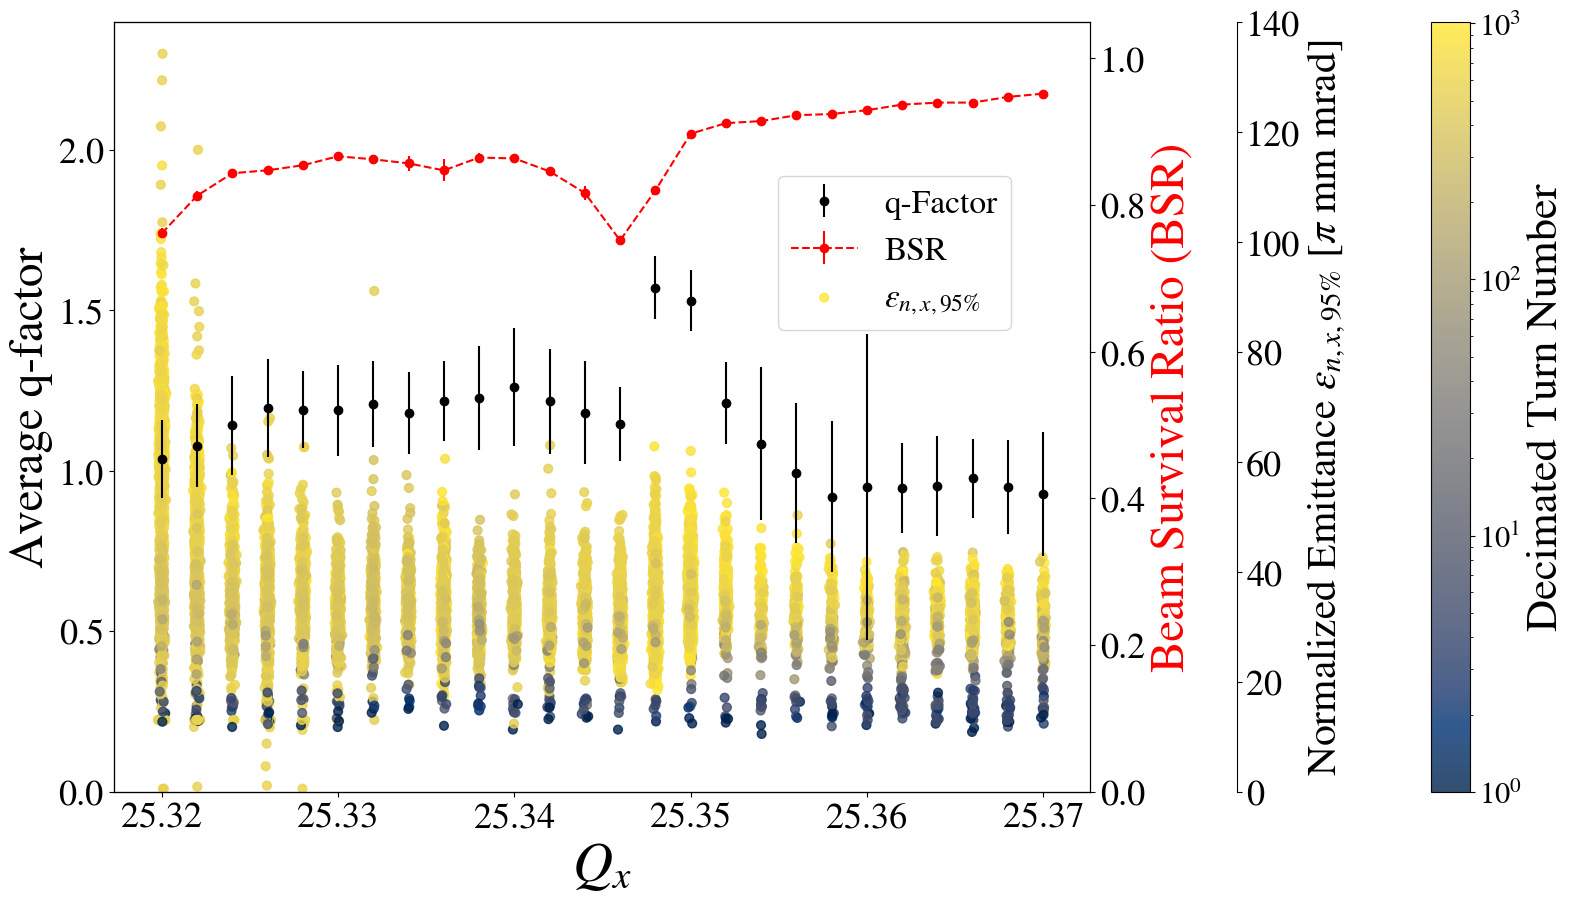
\includegraphics[width=\columnwidth]{chapter6/static14turns_emittance_dampersOFF.png}
    \caption{Static tune scan with beam survival ratio (BSR), average q-factor for the q-Gaussian fits, and beam size $\sigma_x$ at an equivalent intensity of 14 Booster turns or approximately 4.5e10 ppb.}
    \label{fig:static14_q}
\end{figure}

\section{Effect of Transverse Dampers}

\begin{figure}[H]
    \centering
    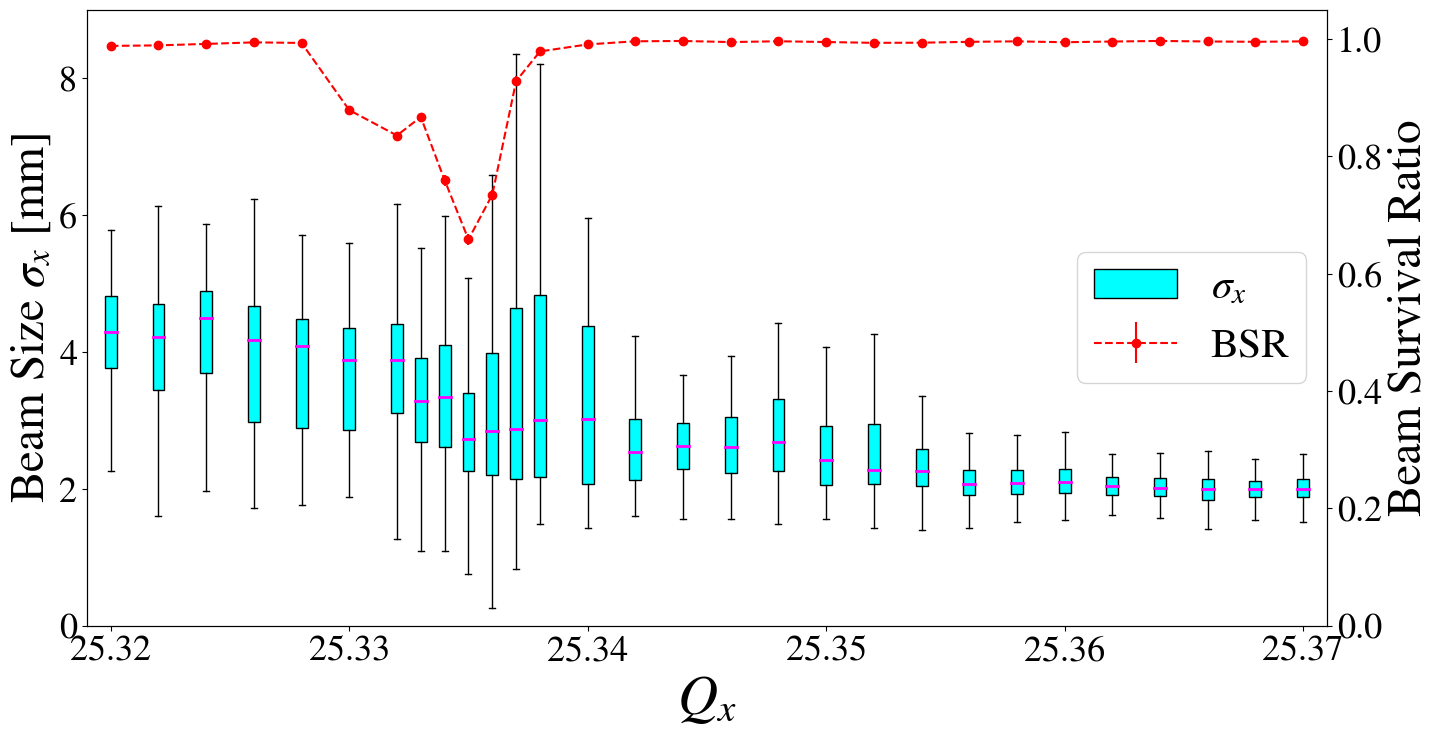
\includegraphics[width=\columnwidth]{chapter6/static2turns_ipm_dampersON.png}
    \caption{Static tune scan with beam survival ratio and IPM data box plots with $3Q_x$ compensation, transverse dampers ON and 2 Booster Turns of equivalent intensity or approximately 0.5e10 ppb.}
    \label{fig:static2_dampersON}
\end{figure}

\begin{figure}[H]
    \centering
    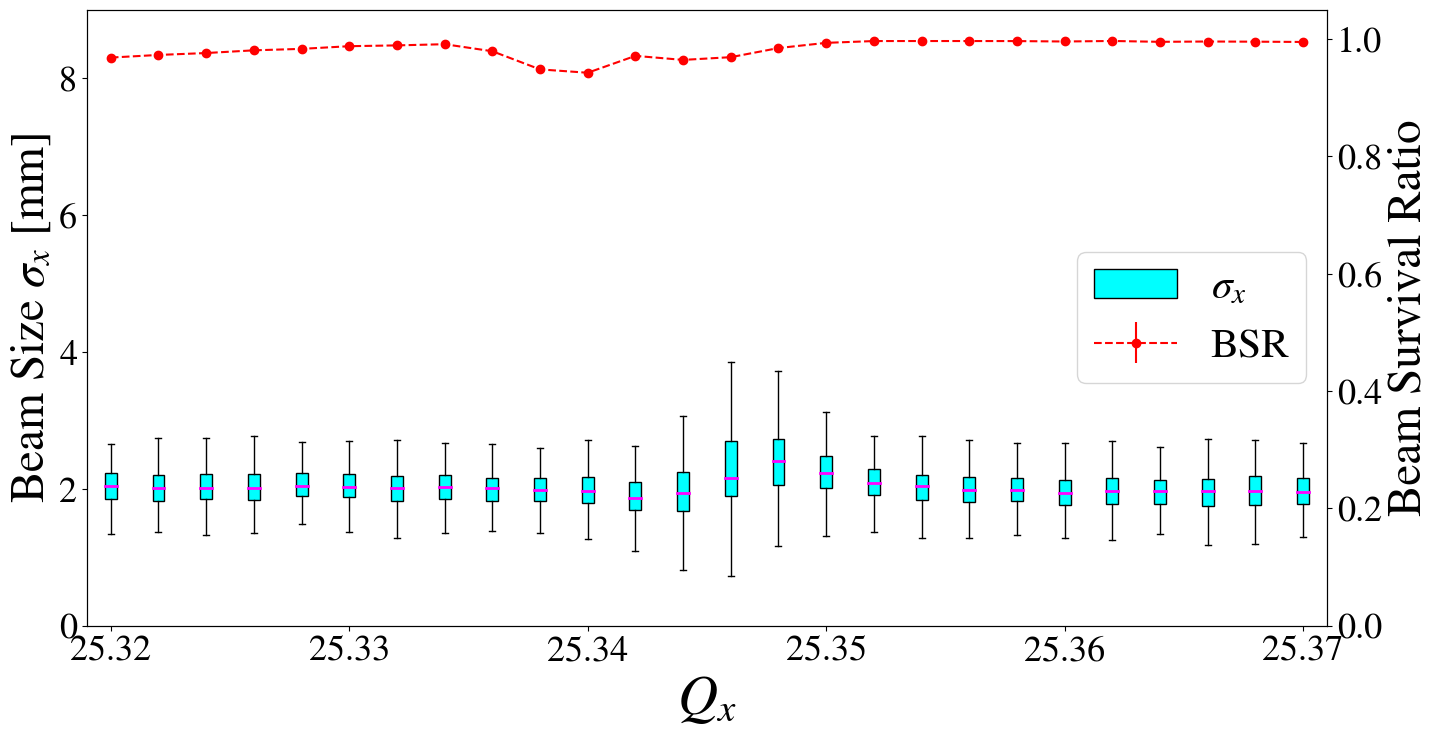
\includegraphics[width=\columnwidth]{chapter6/static2turns_ipm_dampersOFF.png}
    \caption{Static tune scan with beam survival ratio and IPM data box plots with $3Q_x$ compensation, transverse dampers OFF and 2 Booster Turns of equivalent intensity or approximately 0.5e10 ppb.}
    \label{fig:static2_dampersOFF}
\end{figure}

\begin{figure}[H]
    \centering
    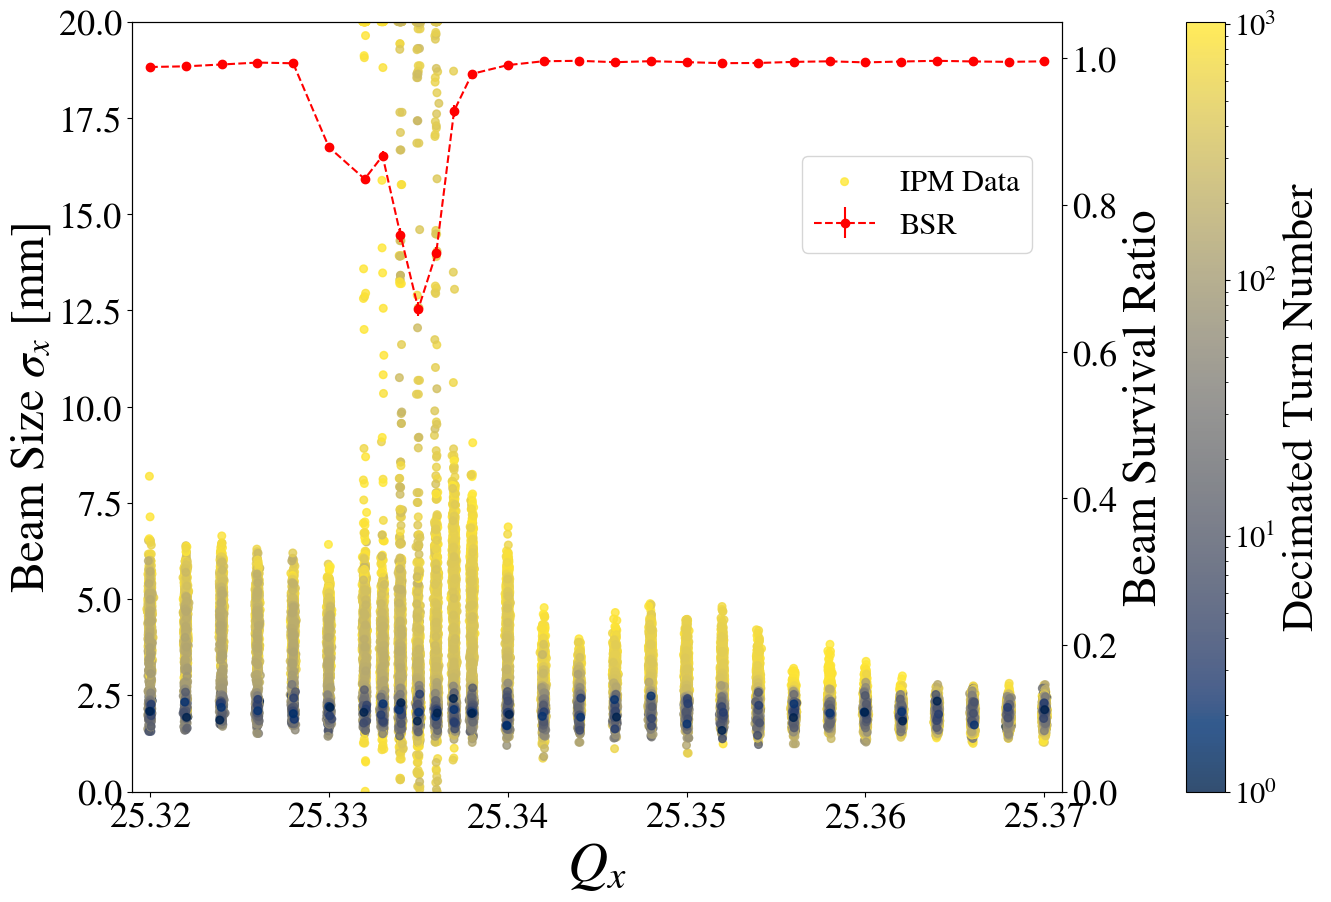
\includegraphics[width=\columnwidth]{chapter6/static2turns_dampersON.png}
    \caption{Static tune scan with beam survival ratio and IPM data scatter plots with $3Q_x$ compensation, transverse dampers ON and 2 Booster Turns of equivalent intensity or approximately 0.5e10 ppb.}
    \label{fig:static2_scatter_dampersON}
\end{figure}